%\red{We assumed access to a library of actions.}

%\textbf{Problem Statement.} 


%In this work, we aim to develop an agent capable of solving long-horizon, goal-reaching tasks in a text-based environment, with only one-time guidance from an LLM prior to any agent training. Specifically, we consider a setting in which the system receives a user-provided natural language instruction \( I \) that specifies the goal $g$ the agent should accomplish, along with additional descriptions of the environment configuration. The agent receives a reward only upon successful completion of the task. We also assume access to a set of successful example instruction–trajectory pairs, denoted as \((I, T)\), generated by humans to help the agent learn how to interact with the environment. Here, \( T = (s_0, a_0, s_1, \ldots, a_{N-1}, s_N)\) represents a state–action sequence. Notably, although we assume these example trajectories successfully reach the ultimate goal, we do not assume that they are optimal due to human errors. 

\begin{figure*}[!t]
    \centering
    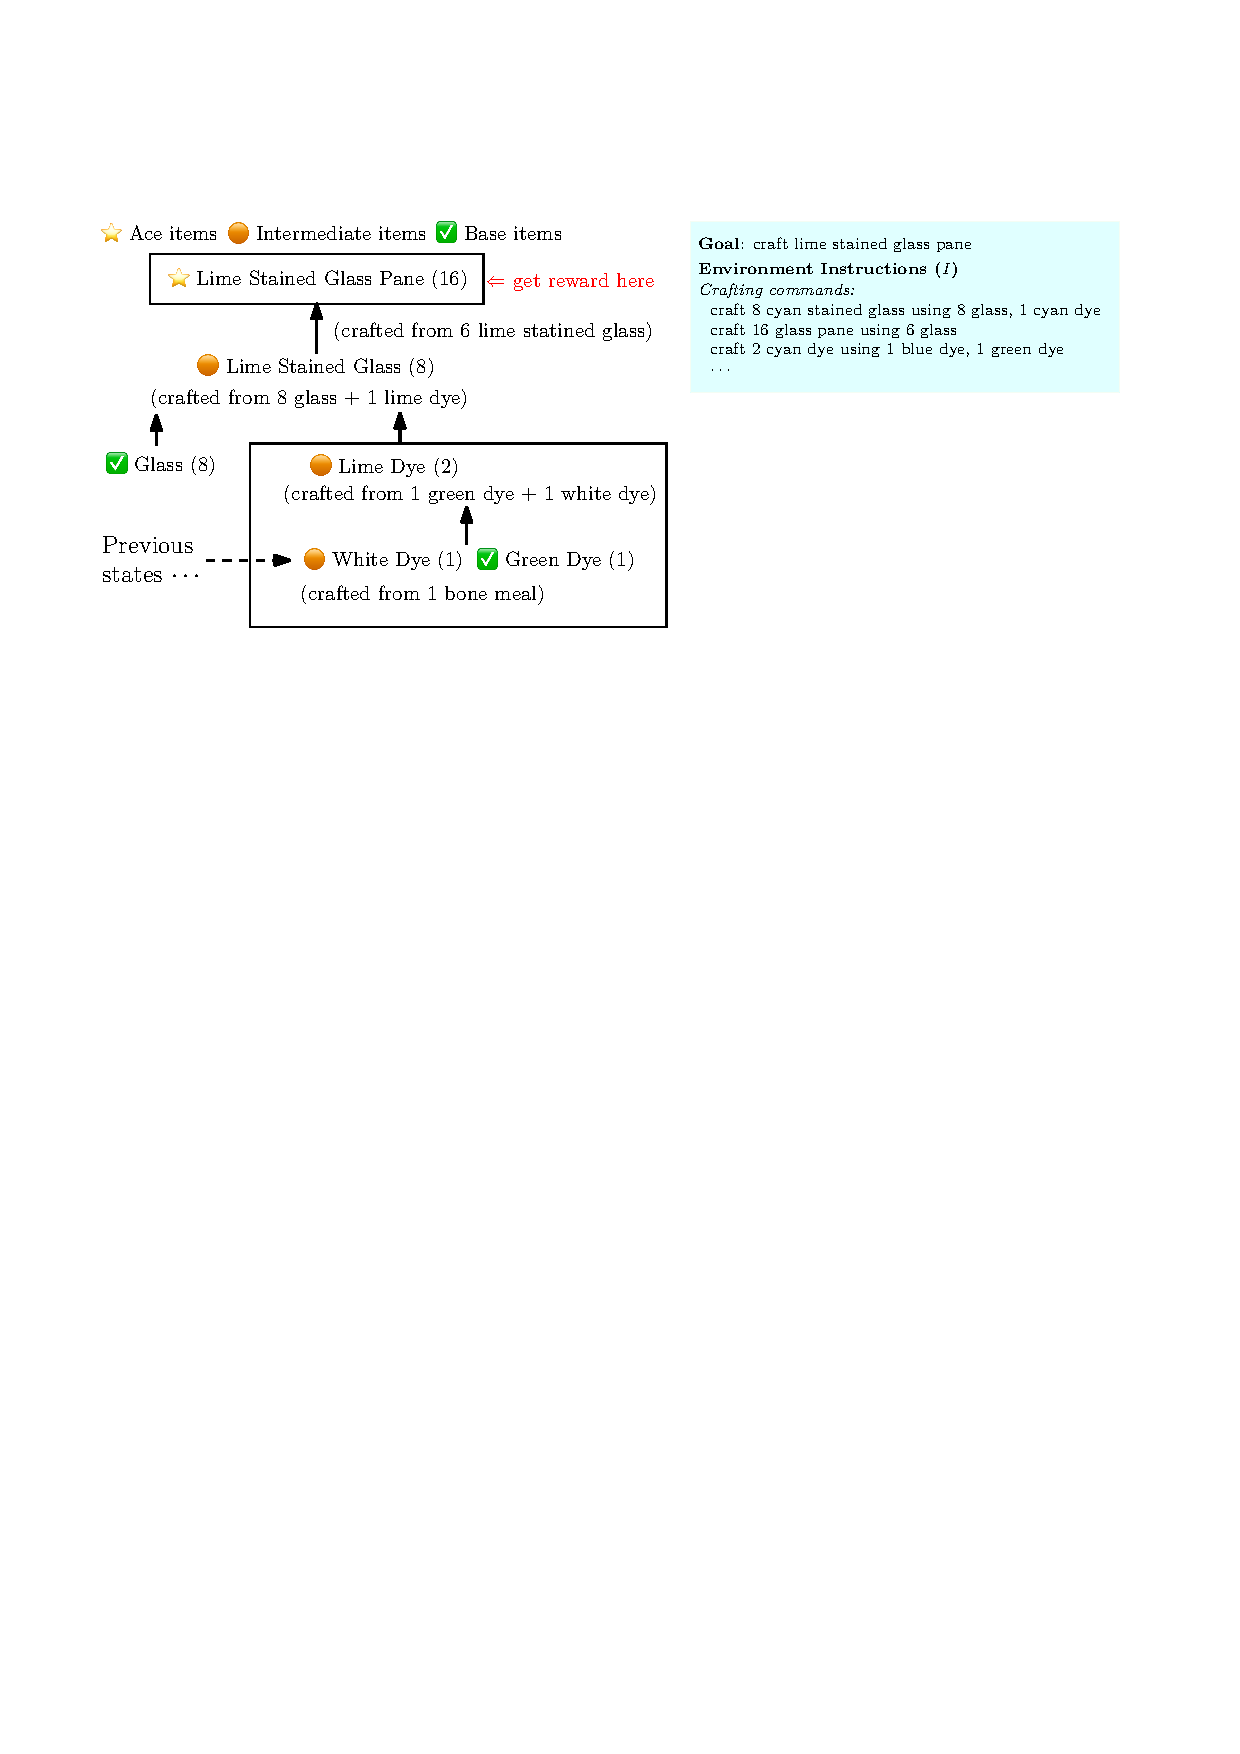
\includegraphics[width=0.8\textwidth]{figs/textcraft_demo.pdf}
    \caption{TextCraft Environment. An example crafting dependency chain for producing the ace item (lime stained glass pane). The agent must gather base items, synthesize intermediate items through the provided crafting commands, and execute the sequence in the correct order to obtain the final reward.
}
    \label{fig:textcraft}
\end{figure*}


In this work, we aim to develop an agent capable of solving long-horizon, goal-reaching tasks in a text-based environment, with only one-time guidance from an LLM prior to any agent training. Specifically, we consider a setting in which the system receives a user-provided instruction that includes a goal  \( g \) that the agent should accomplish, along with additional descriptions of the environment configuration \( I \). The agent receives a reward only upon successful completion of the task. We also assume access to a set of successful example goal-instruction-trajectory tuples,
\(\Sc = \{(g_k, I_k, T_k) \mid k = 1,2,\ldots,N\}\), provided by humans to help the agent learn how to interact with the environment. Each trajectory is defined as
\(T_k = (s_0, a_0, s_1, \ldots, a_{M_k-1}, s_{M_k})\), where each \(a_i\) is the action executed when the agent is in state \(s_i\), thereby forming a sequence of state–action transitions.
Although all example trajectories are assumed to eventually reach the final goal, we do not assume they are optimal, as human demonstrations may include suboptimal or inefficient actions.


%We also assume access to a set of successful example goal-instruction–trajectory tuples, \(\Sc = \{(g_k, I_k, T_k) \mid k = 1,2, \ldots, N\}\), generated by humans to help the agent learn how to interact with the environment. Here, \( T_k = (s_0, a_0, s_1, \ldots, a_{M_k-1}, s_{M_k}) \) represents a state-action sequence. Although these example trajectories are assumed to reach the final goal, we do not assume that they are optimal, as they may contain suboptimal actions due to human errors. 

\textbf{Language Models as One-Time Teacher.} To establish an initial foundation for goal decomposition, an LLM-based planner analyzes the demonstration trajectories and heuristically partitions them into subtrajectories, each ending at a state where a subgoal is deemed achieved. We then train a low-level employee agent to accomplish these short-horizon subgoals, while a high-level manager agent is responsible for proposing them.


To ensure consistent goal decomposition across all trajectories, rather than directly asking the LLM planner to output subtrajectories, we provide it with 50 randomly sampled instruction-trajectory pairs and ask it to propose a Python function \( f_{\text{dc}}(T) \) that systematically decomposes a trajectory \( T  = (s_0, a_0, s_1, \ldots, a_{M-1}, s_M)\) into subtrajectories with associated subgoals. This function is paired with a corresponding subgoal completion function \( f_{\text{sg}}(s, \tilde g) \), which returns \( 1 \) if the subgoal \( \tilde g \) is achieved in state \( s \), and \( 0 \) otherwise. Although the resulting subgoals may be suboptimal and lack interpretability, our empirical study demonstrates that they nevertheless serve as a strong initialization for subgoal decomposition and provide effective guidance for improving the efficiency of long-term planning training. (The prompts used and the generated Python programs are included in \cref{appx:llm_prompt_outputs}.) In pariticular, by applying \( f_{\text{dc}} \), we decompose tuple $(g, I, T)$ into 
\begin{align}
	(\tilde T_k, \tilde g_k, I) \text{\quad with \quad} \tilde T_k = (s_{i_{k-1}}, a_{i_{k-1}}, \ldots, s_{i_{k}}), \quad k = 1, 2, \ldots, N_T, \label{eq:def_subtraj}
\end{align}
where \( i_k \) denotes the index of the state at which subgoal \( \tilde{g}_k \) is achieved (i.e., \( f_{\text{sg}}(s_{i_k}, \tilde{g}_k) = 1 \)), with \( i_0 = 0 \). Here, \(N_T\) denotes the total number of subgoals, and completing the final subgoal \(\tilde{g}_{N_T}\) corresponds to successfully achieving the ultimate goal \(g\).  

For later reference, each subtrajectory in \cref{eq:def_subtraj} is further decomposed into state-action-subgoal-instruction tuples of the form
\((s_{i_{k-1}}, a_{i_{k-1}}, \tilde{g}_k, I)\), which are compiled into the dataset
\(\Phi = \{(s, a, \tilde{g}, I)\}\). In addition, for tuple $(g, I, T) \in \Sc$, let 
\begin{align}
    \Phi_0^{g, I, T} = \big\{\, (s_{i_{k-1}}, \tilde{g}_k, g, I) \;:\; k = 1, 2, \ldots, N_T \,\big\},
\end{align}
where each element of $\Phi_0^{g, I, T}$ corresponds to the initial state of a subtrajectory induced from $T$, paired with its associated subgoal $\tilde{g}_k$, ultimate goal $g$ and instruction $I$. We further define
\begin{align}
	\Phi_0 = \bigcup_{(g, I,T) \, \in \, \Sc} \Phi_0^{g, I, T}. 
\end{align}
\textbf{TextCraft Environment.} In this preliminary work, we use the TextCraft environment \citep{PrasadKHCSBK2024} as the benchmark to evaluate our hierarchical text-based RL framework. TextCraft, inspired by Minecraft, tests an agent's ability to perform compositional reasoning and long-term planning in crafting tasks. As shown in \cref{fig:textcraft}, at the start of each episode, the agent receives a goal $g$ to craft a specific ice item as well as additional instructions $I$ containing a set of available crafting commands. The agent is expected to infer which base items are non-craftable and obtainable from the environment, then act through textual commands -- \texttt{craft} using \texttt{<ingredients>} to produce intermediate or final items, and \texttt{get} to collect the required base materials. The agent tracks its inventory through the textual description of the current state. An episode terminates once the target item is successfully crafted, at which point the agent receives a reward; otherwise, no reward is provided. 
Although the environment appears simple, it is intentionally designed so that crafting the final item requires executing a precise sequence of actions in the correct order, including the creation of multiple intermediate items. This makes TextCraft a suitable testbed for evaluating the effectiveness of hierarchical planning algorithms in an open, purely text-based setting.

%Despite the seemingly simple setup, the environment is intentionally designed to require the agent to execute a precise sequence of actions in the correct order to craft the necessary intermediate items that ultimately lead to producing the final target item. In this sense, it can serve as a good testbed to verify the effectiveness of the proposed algorithm from the long-term planning perspective in an open text world configuration. 


